\chapter{THE LARGE HADRON COLLIDER AND THE CMS EXPERIMENT} \label{lhc-cms}

\section{The Large Hadron Collider}
The Large Hadron Collider is a particle collider near Geneva, Switzerland run by the European Organization for Nuclear Research (CERN). The LHC is the largest and most powerful particle collider ever built, designed to collide protons with a center of mass energy of 14 TeV and a luminosity of $10^{34} {\rm cm^{-2}s^{-1}}$ \cite{LHC}. The luminosity is given by

\begin{equation}
L = \frac{n_{b} f N^{2}_{p} \gamma}{4\pi\epsilon_{n}\beta^{*}}
\end{equation}
where $n_{b}$ is the number of bunches in each ring, f is the frequency for a bunch to circle the ring, ${\rm N_{p}}$ gives the number of protons in a bunch, and ${\rm \gamma}$ is the Lorentz factor. ${\rm \epsilon_{n}}$ is the normalized transverse emittance, a measure of the spread of the beam in momentum and position space. ${\rm \beta^{*}}$ measures the focus of the beam at the interaction point, and ${\rm \epsilon_{n}\beta^{*}}$ represents the transverse area at the point of interaction. The large luminosity at the LHC is characterized by a high frequency of bunch crossings (every 25 ns) with about 10$^{11}$ protons in each bunch packed as densely as possible, resulting in a high rate of collisions. With many collisions at high energy, the detectors can collect enough events from yet unexplored energy regimes to discover new physics, to verify old physics, or to discard certain theories of physics. 

The collider itself is 26.7 km in circumference and 45-170 m underground. 8.3 T supercooled, superconducting magnets operating at 2 K steer the high energy proton beams. In order to save money, the LHC not only reuses the tunnels of a previous collider, the Large Electron Positron Collider (LEP), but also reuses older accelerators which were state of the art at their time. These older accelerators ramp up the energy of the protons and inject them into the LHC. All of this together makes up the CERN accelerator complex.

\begin{figure}[h!]
  \centering
  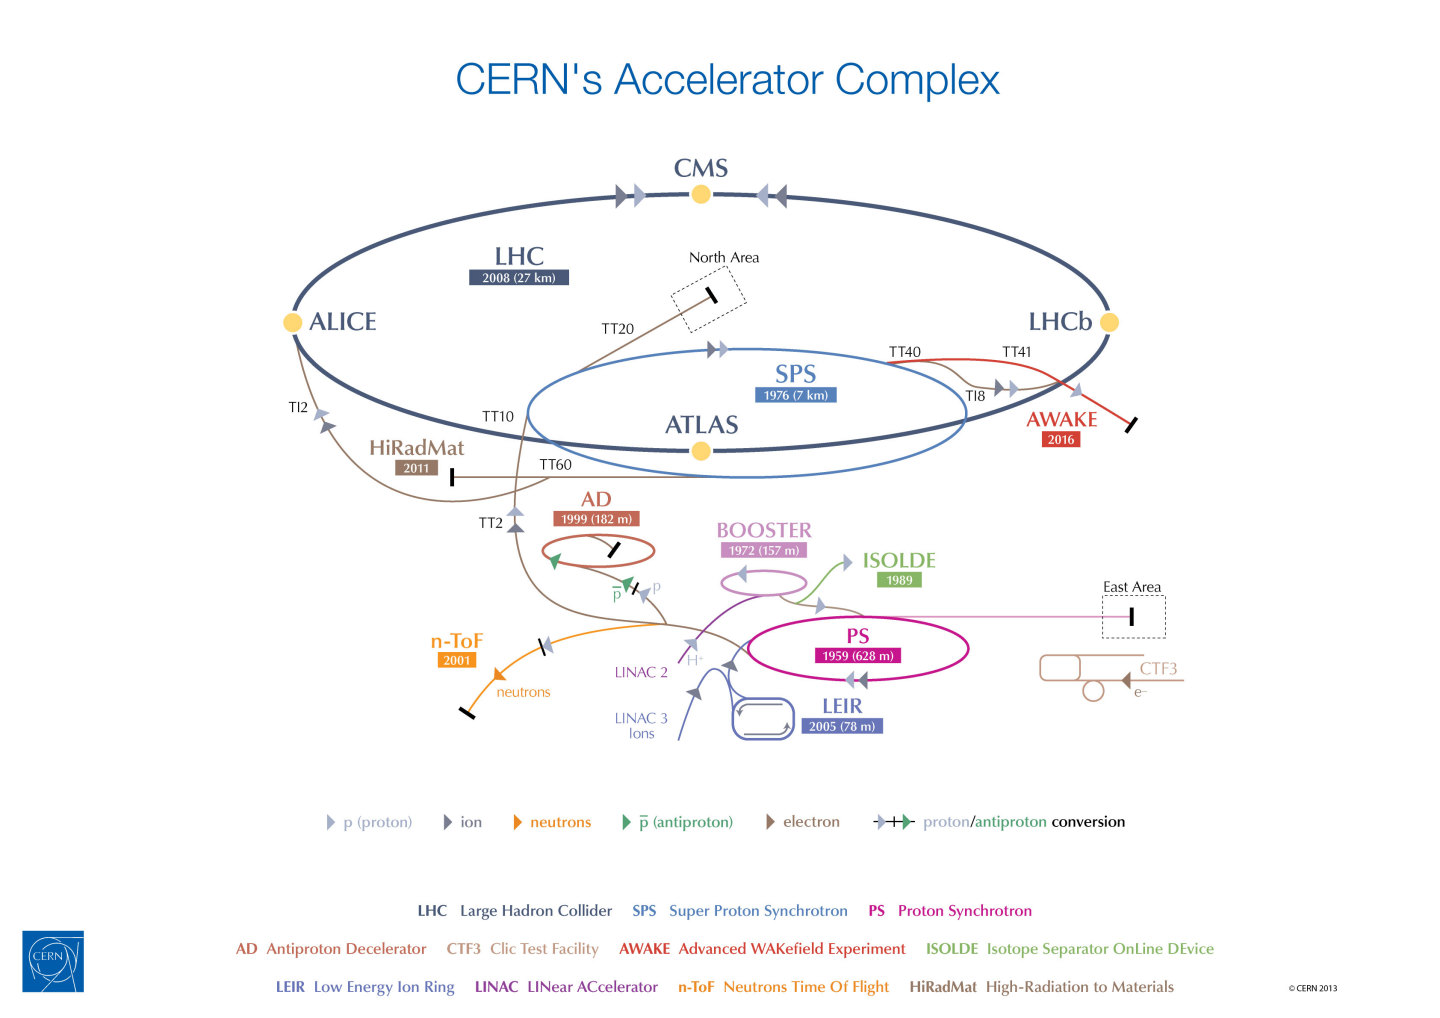
\includegraphics[width=6in]{images/cern_accel_complex.png}
  \caption
   {The CERN Accelerator Complex \cite{cernaccelcomplex}}
  \label{fig:cernaccel}
\end{figure}

First, the protons are created from a source of Hydrogen gas. The hydrogen atoms of the gas are placed into a large electric field that separates the atoms into unbound protons and electrons. The protons are then sent to a radio frequency quadrapole which focuses the protons and accelerates them. The radio frequency field is stronger for the protons in the back than in the front and consequently squeezes them into a tighter bunch. The protons then proceed to a linear accelerator, LINAC2, where they are accelerated to 50 MeV or 5\% of the speed of light (c). The protons then enter a series of synchrotrons. A synchrotron is a device that accelerates particles by guiding them around a fixed circular path with a magnetic field while boosting their speed with an electric field as they pass a certain point. Since a faster particle bends less in the same magnetic field, the magnetic field strength is synchronized with the speed of the accelerating particles to keep them in the fixed circular path. 

After LINAC2, the protons enter the first of the synchrotrons, the Proton Synchrotron Booster (PSB) accelerating the protons to 1.4 GeV (0.81c). From here the protons are injected into the Proton Synchrotron (PS) and accelerate to 25 GeV (0.999c). The PS then injects the protons into the Super Proton Synchrotron (SPS) further accelerating them to 450 GeV (0.99999c). Finally the protons are injected into the LHC where they accelerate up to 6.5 TeV (0.99999999c). Once accelerated to the appropriate collision energy, the proton beams are made to collide in the different detectors located around the ring. By colliding enough protons at large enough energies, it is possible to probe corners of physics that have never been seen before. The two general purpose detectors at the LHC, ALTAS and CMS, are used to look for signs of new physics like the Higgs boson, dark matter, and extra dimensions by measuring the energy, the momentum, and the paths of the particles coming out of the collisions.

\section{The Compact Muon Solenoid}

The Compact Muon Solenoid (CMS), located in Cessy, France, is 21.6 m long, 15 m in diamater, and weighs more than the Eiffel Tower. Not only is the CMS detector a massive and complex device it's also run by a huge collaboration involving approximately 3,800 people from 200 institutes spanning 43 different countries \cite{cmscollab}. The greatest achievement of the collaboration to date is the discovery of a Higgs like particle in 2012, a feat shared with ATLAS.

\begin{figure}[h!]
  \centering
  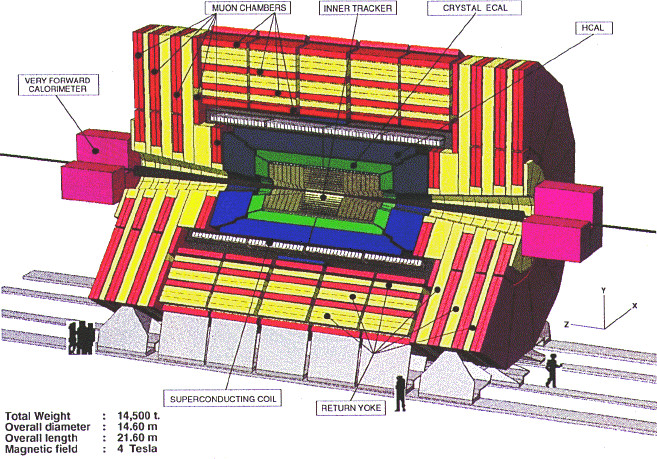
\includegraphics[width=4in]{images/CMSdetc3D.jpg}
  \caption
   {The CMS detector \cite{cmsweb}}
  \label{fig:cmsdet3d}
\end{figure}

CMS was built primarily to look for the Standard Model Higgs and signs of Beyond Standard Model (BSM) physics like Supersymmetry, extra dimensions, or new heavy weak bosons \cite{tdr}. Because BSM and Higgs decays to muons and electrons often have the highest signal to background ratio, CMS is designed to identify and measure these particles with a high accuracy. A high signal to background ratio means that the events of interest have fewer look-alikes. Jets \footnote{When a quark or gluon is created, it pulls other quarks from the vacuum in order to maintain colorlessness. The result is a cone of colorless particles called a jet.} and photons are measured to a high degree of accuracy as well. In order to measure the energy, momentum, and location of the different types of particles CMS deploys a variety of subdetectors working in concert. The defining feature of the detector is an extremely powerful solenoid which enables the accurate measurement of momentum for charged particles. The tracker and calorimeters fit snugly within the 6 m diameter solenoid. The muon detectors reside outside the magnet but within the return yoke.

\subsection{Silicon Tracker}
The 3.8T magnetic field inside the solenoid enables the tracker to measure the transverse momentum of charged particles based upon the curvature of the track. Charged particles with lower transverse momentum ($p_{t}$) bend more in a magnetic field than high $p_{t}$ particles. As such, a measurement of the deviation of a curved track from a straight line, the sagitta, can be used to measure the curvature and determine the momentum \cite{pdgreview}.

\begin{equation}
p_{t} \cong \frac{L^{2}qB}{8s}
\end{equation}
Here L is the length of the straight line between the first and last position measurments, q is the charge of the particle, B is the magnetic field, and s is the sagitta.
\begin{figure}[h!]
  \centering
  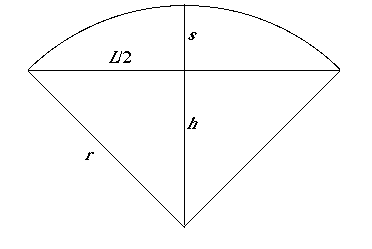
\includegraphics[width=3in]{images/sagitta.png}
  \caption
   {The sagitta measurement}
  \label{fig:sagittadrawing}
\end{figure}
The equation for the error in the momentum measurement shows that a higher magnetic field enables better $p_{t}$ resolution, illuminating the design choice for a powerful magnet.
\begin{equation}
\frac{\delta p_{t}}{p_{t}} \propto \frac{p_{t}}{L^{2}B} 
\end{equation}

The silicon tracker is made of tiny reverse biased bipolar diodes. When a charged particle travels through one of these diodes, the particle liberates electron hole pairs beyond the electrostatic equilibrium, and a current flows. The tracker needs to be small enough such that the particles traveling through it don't deposit much energy. Energy deposition in the tracker would throw off energy measurements in the calorimeters. This means that the tracker needs to be smaller than a few radiation lengths \footnote{the length scale over which an electron deposits a substantial amount of energy into the material}. At CMS, the thickest part of the tracker is one radiation length. The tracker is placed nearest the collision point in order to identify primary and secondary vertices and to measure the momentum of particles before they are tainted by interactions with other detectors. \footnote{A vertex is an interaction point from which a set of particles emanate.} Being so near the collision point, the silicon tracker is bombarded by a constant flux of high intensity radiation. As such, the tracker is carefully designed to be robust to this radiation rich environment.

\FloatBarrier
\subsection{Calorimeters}
The Electromagnetic Calorimeter (ECAL) is right outside the tracker and its main goal is to measure the energy of electrons and photons. It's designed to contain entire electromagnetic showers for these particles and is consequently many radiation lengths thick. The ECAL is made of lead tungstenate scintillating crystals which release an amount of light proportional to the energy deposition. The light is collected and the total energy is calculated. The separation into individual crystals allows some spatial resolution as well. Particles with larger mass deposit less energy per unit distance into a solid. Many of the hadronic particles make it through the ECAL for this reason.

\begin{figure}[h!]
  \centering
  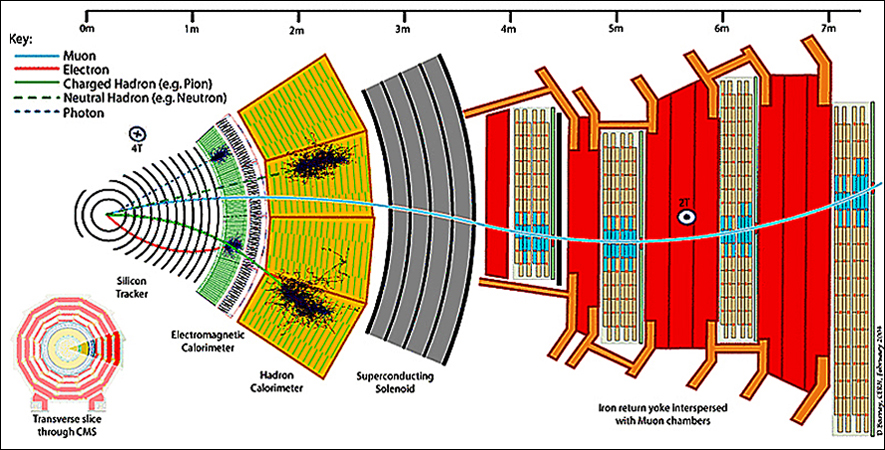
\includegraphics[width=4in]{images/cms_slice.jpg}
  \caption
   {A slice of the CMS detector \cite{cmsweb}}
  \label{fig:cmsdetslice}
\end{figure}

The HCAL is placed outside the ECAL to collect the energy of the particles that survived the other subsystems. The surviving particles that interact strongly with the HCAL are mostly hadronic particles from jets. The HCAL works in a similar manner to the ECAL except that layers of plastic scintillating material are interspersed with layers of a dense passive absorber like brass or steel. The density of the passive absorber increases the chance of interaction and shower production thus reducing the total length of the hadronic shower and enabling the measurement of the total energy for most of the cascades. Again, the scintillation light is collected to determine the energy. If the ECAL and HCAL were placed outside the magnet the particles would interact with the solenoid material before entering the calorimeters, throwing off their measurements. The showers in the calorimeters are a consequence of the electromagnetic and strong forces, which means that particles without these interactions pass through the materials undetected, e.g. neutrinos or BSM weakly interacting particles. Since the momentum in an interaction is conserved, any imbalance means that some particles escaped the detector. If there is an excess of missing momentum beyond the amount expected due to neutrinos this may indicate the existence of dark matter or some other BSM particle. In order to measure the missing energy correctly, it's important that the HCAL is built without any gaps and that it is dense enough to collect the energy of the strongly and electrically interacting particles.

While the momentum resolution in the tracker is proportional to the momentum, the energy resolution in the calorimeters decreases with increasing energy \cite{pdgreview}.
\begin{equation}
\frac{\delta E}{E} = \sqrt{\left(\frac{S}{\sqrt{E}}\right)^2 + \left(\frac{N}{E}\right)^2 + C}
\end{equation}
The first term in the square root describes statistical fluctuations. The energy measured is proportional to the number of photons captured which has poisonnian fluctuations and the error (${\rm \delta E}$) for this term is $\propto \sqrt{{\rm E}}$. The second term describes noise in the electronics whose error is energy independent, and the last term describes the errors in energy calibration which are proportional to energy.

\FloatBarrier
\subsection{Muon System}
Neutrinos aren't the only Standard Model particles that make it through the tracker, ECAL, and HCAL. Muons have a relatively long lifetime $\sim 10^{-6} s$  with $c\tau \sim 100 m$. The large gamma factor associated with the large energies of the muons at the LHC, in combination with their long lifetime, enables them to travel hundreds of kilometers on average, well through the entire CMS detector before decaying. Muons are charged so their tracks show up in the tracker and some energy is deposited in the calorimeters but, muons are so much more massive than electrons that the energy deposition in the ECAL is minimal. Making it through the ECAL, the muons enter the HCAL. The HCAL is designed to stop strongly interacting hadronic particles and collect their energy. But muons don't interact with the strong force, and they make it through the HCAL as well. This enables the muon system to be placed outside the magnet.

The muon system consists of a few different types of detectors which all involve the same basic principle. The charged muon ionizes some gas and the ionized particles are attracted to charged surfaces initiating a current in the surfaces. With a large enough voltage differential between the charged surfaces the the ionized particles may gain enough kinetic energy to further ionize other atoms in the gas initiating an avalanche effect which reduces the need for signal amplification later. The muon system uses this strategy in the different detectors. The types of detectors in the muon system are the Cathode Strip Chambers (CSC), the Drift Tubes (DT), and the Resistive Plate Chambers (RPC) \cite{tdr}.

\begin{figure}[h!]
  \centering
  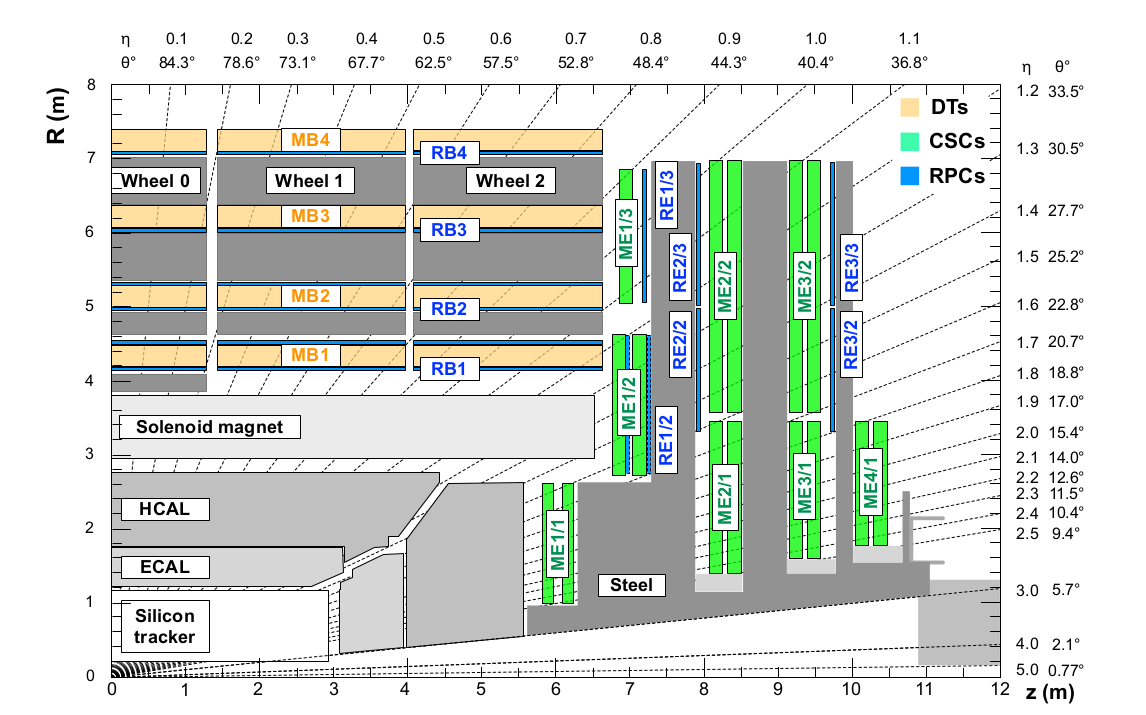
\includegraphics[width=5.5in]{images/muon_system.png}
  \caption
   {A Look at the Muon System \cite{muonsys}}
  \label{fig:muonsysfig}
\end{figure}

\FloatBarrier
\subsubsection{Drift Tubes}

The drift tubes are located in the barrel portion of CMS. Throughout the majority of the barrel the magnetic field is basically uniform. The drift tubes have aluminum plates on the top and bottom separated by aluminum I-beams as shown in Figure ~\ref{fig:dt}. A wire acts as the anode and the I-beams are the cathodes. The tubes are designed to provide a constant drift velocity throughout each tube.
\begin{figure}[h!]
  \centering
  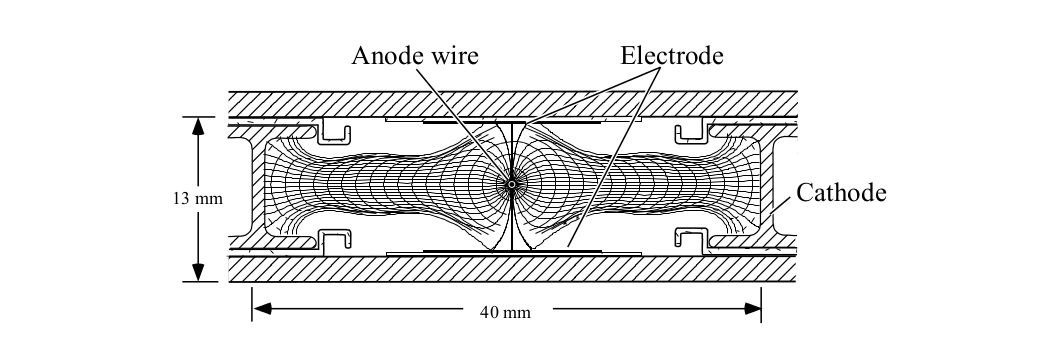
\includegraphics[width=4in]{images/DT.png}
  \caption
   {A Drift Tube \cite{mutdr}}
  \label{fig:dt}
\end{figure}

When a charged particle flies through the tube, it ionizes the gas inside. The electrons drift at constant velocity to the anode. The distance from the anode is deduced from the drift time, utilizing the fact that the ionized electrons drift with a constant velocity. This calculation does however require a reference time. In each chamber the drift tubes are placed in layers and the average crossing time in the chamber is used as the reference time.

\FloatBarrier
\subsubsection{Cathode Strip Chambers}

The CSCs are located in the endcaps of the detector which range in $|\eta|$ from 0.8 to 2.4. The nonuniform magnetic field in the endcaps would adversely affect the drift times in the DTs, so the endcaps use CSCs instead. In this system, there are oppositely charged strips and wires running roughly perpendicular to eachother.

\begin{figure}[h!]
  \centering
  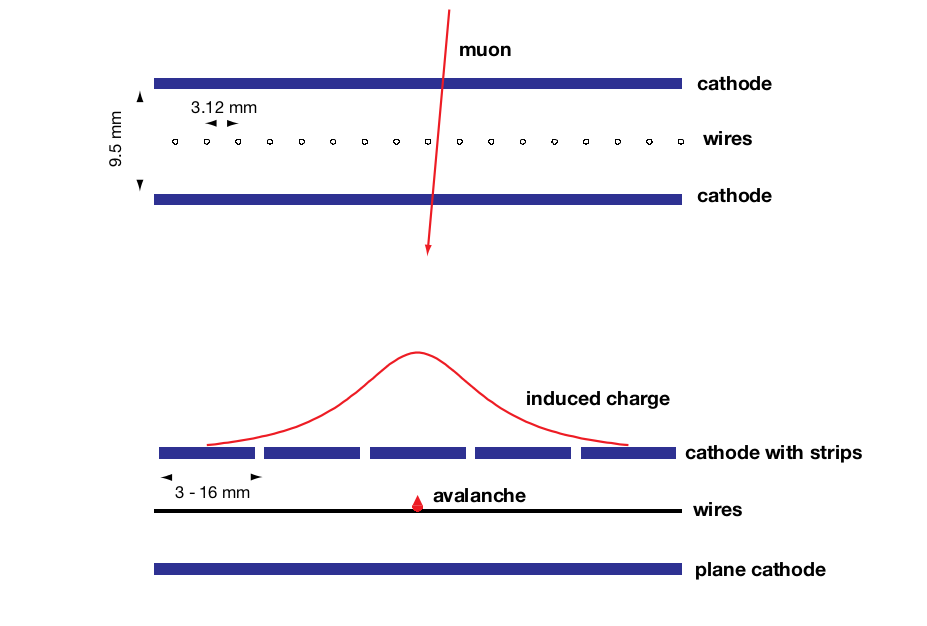
\includegraphics[width=4in]{images/CSC.png}
  \caption
   {A Cathode Strip Chamber \cite{mutdr}}
  \label{fig:csc}
\end{figure}
When a muon flies through a CSC, it induces charge on the wires and the strips and ionizes gas in the chamber. The ionized particles in the gas float to the charged strips and wires initiating a current in those components. The induced charge from the muon itself also contributes to the currents. The most intense currents are those associated with the location of the muon, and the position resolution in the $\phi$ direction is roughly 100 ${\rm \mu m}$.

\FloatBarrier
\subsubsection{Resistive Plate Chambers}

The RPCs are located both in the barrel and in the endcaps. The RPCs have excellent timing resolution on the order of 1 ns. The RPCs use their excellent timing resolution to determine each particle's bunch crossing of origin. The accurate and rapid timing information helps with the online selection of muons, a huge priority for CMS considering that many interesting collisions produce muons. For this reason, the RPCs focus on efficient online selection of muons instead of accurate offline reconstruction \cite{cmsexp}.

In this way, the RPCs complement the DTs and CSCs. The RPCs consist of two high resistance parallel plates surrounding a volume of gas. The outsides of the plates are painted with graphite paint forming the electrodes. A large voltage differential is kept between the electrodes. When a charged particle crosses the plates it induces an electrical discharge in the plates which remains localized in time and space due to the large resistivity.

\subsection{Trigger System}
Collision events come at a rate of 10 MHz with each event taking up roughly a MB of information. If the detector had to store all of the information from each event this would amount to pushing terabytes of information into a storage system every second, which is remarkably infeasible. To deal with this issue, CMS utilizes a trigger system which selects only interesting events and cuts the rate down from 40 MHz to 1 KHz \cite{cmsexp}. Since bunch crossings happen every 25 ns, the trigger needs to operate at an incredibly high rate.

CMS tackled this issue by dividing the trigger into different tiers. The Level-1 Trigger is the first stage of the trigger system made from custom hardware which can operate at fantastic speed. The Level-1 Trigger reduces the rate from 40 MHz to 100 KHz. The events passing the L1 Trigger move onto the High Level Trigger (HLT) which further reduces the rate to 1 KHz. Due to the lower input rate the HLT can operate in software.

\subsubsection{Level-1 Trigger}

The Level-1 (L1) Trigger is made of up different subsystems that work together to decide whether to keep the data from a beam crossing for further processing. The University of Florida works with the Level-1 muon trigger system, the Endcap Muon Track Finder (EMTF) in particular. The muon system needs to determine the transverse momenta of muons and their location and choose the best candidates. Each of the different muon detectors have their own local triggers which send their best muon tracks to the Global Muon Trigger (GMT). The GMT chooses the best muon candidates from that set and passes these on to the Global Trigger (GT). The GT combines the information from the calorimeter triggering system and uses the combined information to check whether the bunch crossing should be sent to the HLT or discarded. The L1 Trigger has many different trigger criteria defining separate triggers. These pass/fail information from the separate triggers define the trigger bits. If an event passes any of the triggers then it is forwarded for further processing.

\begin{figure}[h!]
  \centering
  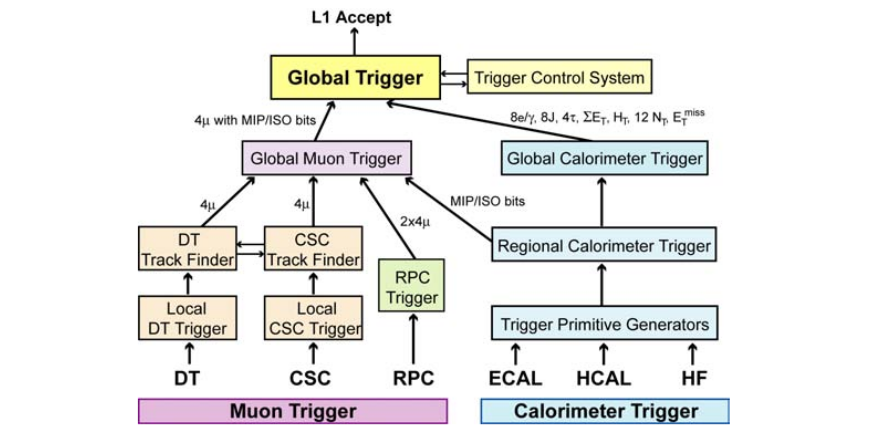
\includegraphics[width=5in]{images/L1_Trigger.png}
  \caption
   {The L1 Trigger Architecture \cite{cmsexp}}
  \label{fig:l1trigarch}
\end{figure}

The Track Finders (TF) play an important role in the L1 Trigger system. The EMTF combines the location and direction information from the different CSC stations into muon tracks and calculates the transverse momenta for the different tracks. The EMTF chooses the best candidates (highest momentum and highest quality) to send to the GMT. The Drift Tube Track Finder (DTTF) performs a similar process for muons in the DT system. The RPC system calculates the location and direction and forms tracks in the same stage. In the process the RPC trigger system assigns transverse momenta and quality, and like the others chooses the best tracks to send to the GMT.
